\documentclass[tikz, border=20pt]{standalone}
\usepackage{tikz}
\usetikzlibrary{arrows.meta, shapes.geometric}

\begin{document}
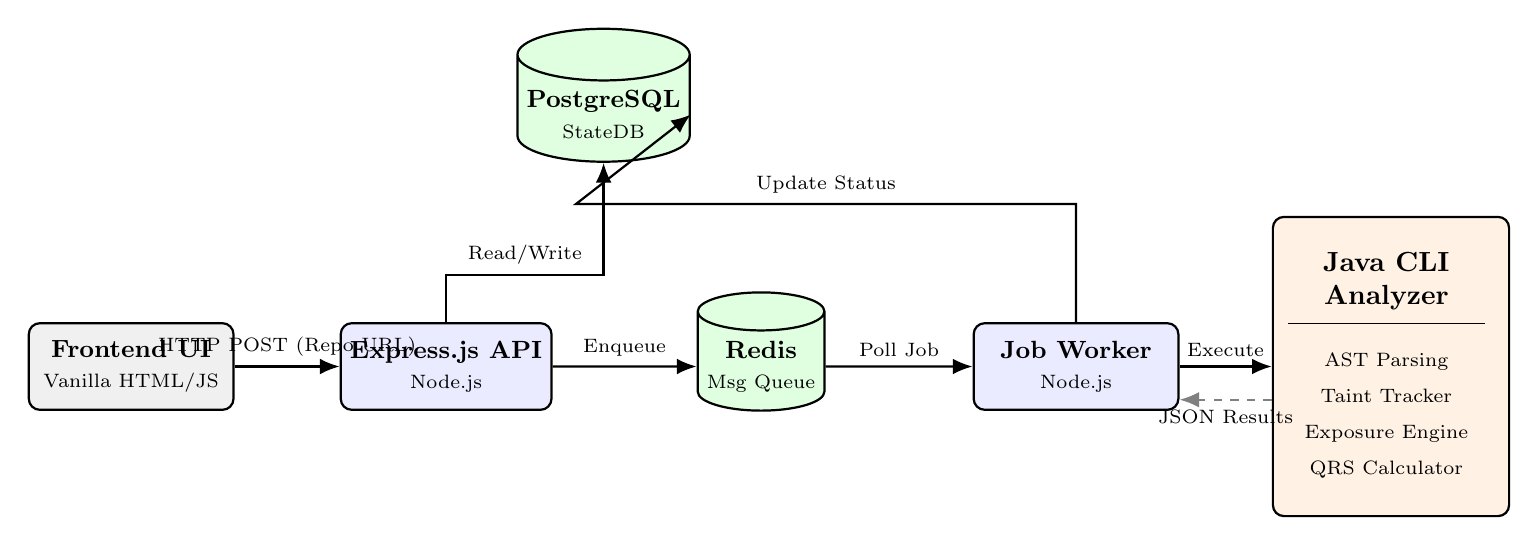
\begin{tikzpicture}[
    box/.style={
        draw, rectangle, rounded corners=4pt,
        minimum width=2.6cm, minimum height=1.1cm,
        align=center, font=\small, thick, fill=blue!8
    },
    db/.style={
        draw, cylinder, shape border rotate=90, aspect=0.3,
        minimum width=1.6cm, minimum height=1.4cm,
        align=center, font=\small, thick, fill=green!12
    },
    arr/.style={-{Latex[length=2.5mm, width=2mm]}, thick},
    darr/.style={-{Latex[length=2.5mm, width=2mm]}, thick, dashed, gray}
]

%% ---- Nodes at explicit (x,y) positions ----

% Main horizontal pipeline (y=0)
\node[box, fill=gray!12]   at ( 0, 0) (fe)       {\textbf{Frontend UI}\\{\scriptsize Vanilla HTML/JS}};
\node[box]                 at ( 4, 0) (api)      {\textbf{Express.js API}\\{\scriptsize Node.js}};
\node[db]                  at ( 8, 0) (redis)    {\textbf{Redis}\\{\scriptsize Msg Queue}};
\node[box]                 at (12, 0) (worker)   {\textbf{Job Worker}\\{\scriptsize Node.js}};

% Analyzer box on right (y=0, taller)
\node[draw, rectangle, rounded corners=4pt, thick, fill=orange!10,
      minimum width=3.0cm, minimum height=3.8cm, align=center]
                           at (16, 0) (analyzer) {
    \begin{tabular}{c}
        \textbf{Java CLI}\\
        \textbf{Analyzer}\\[3pt]
        \hline\\[-5pt]
        {\scriptsize AST Parsing}\\[1pt]
        {\scriptsize Taint Tracker}\\[1pt]
        {\scriptsize Exposure Engine}\\[1pt]
        {\scriptsize QRS Calculator}
    \end{tabular}
};

% PostgreSQL floats above API (y=3)
\node[db] at (6, 3.2) (pg) {\textbf{PostgreSQL}\\{\scriptsize StateDB}};

%% ---- Arrows ----

% 1. Frontend -> API  (straight horizontal)
\draw[arr] (fe.east) -- node[above, font=\scriptsize]{HTTP POST (Repo URL)} (api.west);

% 2. API -> Redis  (Enqueue)
\draw[arr] (api.east) -- node[above, font=\scriptsize]{Enqueue} (redis.west);

% 3. Redis -> Worker  (Poll Job)
\draw[arr] (redis.east) -- node[above, font=\scriptsize]{Poll Job} (worker.west);

% 4. Worker -> Analyzer  (Execute subprocess)
\draw[arr] (worker.east) -- node[above, font=\scriptsize]{Execute} (analyzer.west);

% 5. Analyzer -> Worker  (JSON Results, dashed, offset below)
\draw[darr] ([yshift=-12pt]analyzer.west) --
    node[below, font=\scriptsize, black]{JSON Results}
    ([yshift=-12pt]worker.east);

% 6. API -> PostgreSQL  (vertical up, Read/Write)
\draw[arr] (api.north) -- ++(0, 0.6) --
    node[above, font=\scriptsize]{Read/Write}
    ++(2, 0) -- (pg.south);

% 7. Worker -> PostgreSQL  (Update Status)
%    Go up from worker, travel left above the pipeline, enter postgres from right
\draw[arr] (worker.north) -- ++(0, 1.5) --
    node[above, font=\scriptsize]{Update Status}
    ++(-6.35, 0) -- (pg.east);

\end{tikzpicture}
\end{document}
